%auto-ignore
\documentclass{standalone}

\usepackage{graphicx}
\usepackage{tikz}

\begin{document}
\begin{tikzpicture}
\node[inner sep=0pt,label={[yshift=0.95cm]\textbf{find} \#1}]
(clip1) at (0,0)
	{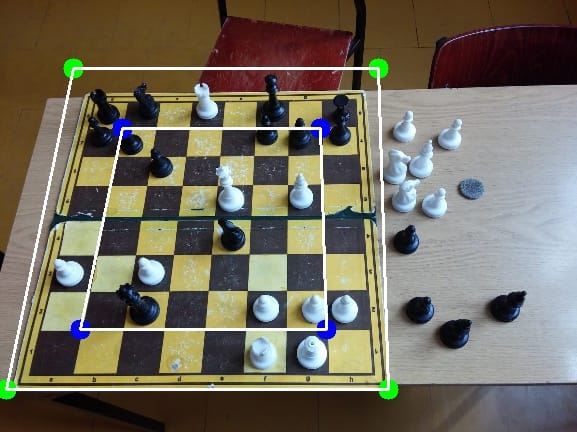
\includegraphics[width=.25\textwidth]{figure2_3.jpg}};
\node[inner sep=0pt,label={[yshift=0.50cm]\textbf{analyze} \#2}]
(clip2) at (6,0)
	{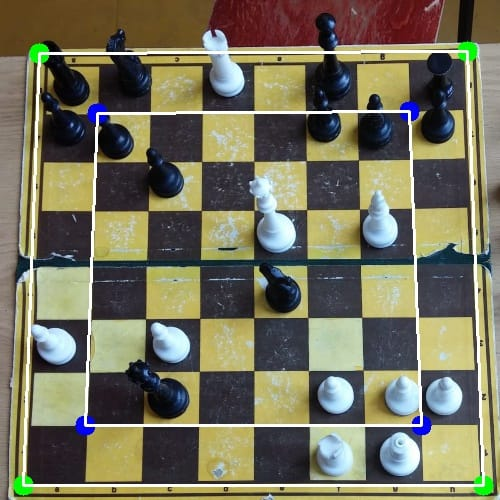
\includegraphics[width=.25\textwidth]{figure2_2.jpg}};
\node[inner sep=0pt,label={[yshift=0.50cm]\textbf{catch} \#3}]
(clip3) at (12,0)
	{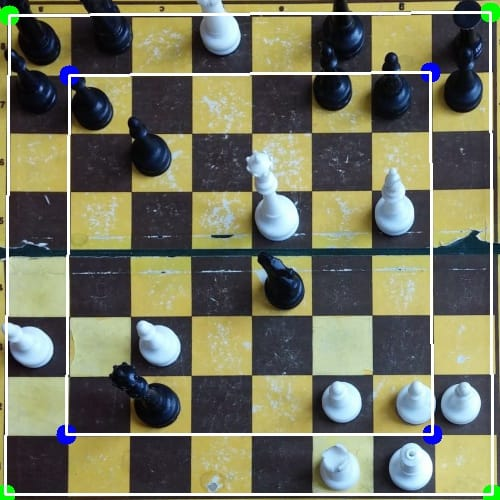
\includegraphics[width=.25\textwidth]{figure2_1.jpg}};
\draw[->,thick,shorten >=6pt,shorten <=6pt] (clip1) -- (clip2)
	node[midway,fill=white] {padcrop};
\draw[->,thick,shorten >=6pt,shorten <=6pt] (clip2) -- (clip3)
	node[midway,fill=white] {padcrop};
\end{tikzpicture}
\end{document}
